\section{ЭКСПЕРИМЕНТАЛЬНОЕ ИССЛЕДОВАНИЕ}

\subsection{Условия проведения экспериментов}

Все эксперименты проводились в облачной среде Google Colab Notebooks с использованием графического ускорителя NVIDIA Tesla T4, 16~ГБ видеопамяти. Программное окружение: Python~3.10, PyTorch~2.x с поддержкой CUDA, библиотеки torchvision, opencv-python, pandas, scikit-learn, iterative-stratification.

Размер пакета при обучении --- 32 примера, размер изображения --- $320 \times 320$ пикселей, число эпох --- 50 с ранней остановкой. Время обучения одной эпохи составляет около 60 секунд, полный цикл обучения занимает около 30--50 минут в зависимости от срабатывания ранней остановки.

Воспроизводимость обеспечивается фиксированным значением \texttt{random\_state} = 42 для всех источников случайности: разбиения выборки, инициализации весов сети, перемешивания данных и взвешенного сэмплирования.

\subsection{Метрики качества}

Для оценки качества модели применяются три варианта F1-меры~\cite{f1-score}:

\begin{itemize}
    \item F1\textsubscript{micro} --- F1, вычисленная по агрегированной матрице ошибок с одинаковым весом каждого предсказания. В целом, можно сказать близка к accuracy и отражает общую долю правильных предсказаний;
    \item F1\textsubscript{weighted} --- среднее F1 по классам с весами, пропорциональными количеству примеров каждого класса в выборке. Учитывает редкость классов, не штрафуя избыточно за их пропуск;
    \item F1\textsubscript{macro} --- среднее значение F1 по классам каждого признака с равными весами для всех классов независимо от их частоты. Чувствительна к качеству модели на минорных классах.
\end{itemize}

Формально метрики определяются следующим образом. Для каждого класса $c$ определяются количества истинно положительных (TP$_c$), ложно положительных (FP$_c$) и ложно отрицательных (FN$_c$) предсказаний. Точность (precision) и полнота (recall) для класса $c$:  

\begin{equation}
P_c = \frac{\text{TP}_c}{\text{TP}_c + \text{FP}_c}, \quad R_c = \frac{\text{TP}_c}{\text{TP}_c + \text{FN}_c}
\end{equation}

F1\textsubscript{micro} агрегирует TP, FP, FN по всем классам перед вычислением:
\begin{equation}
\text{F1}_{\text{micro}} = \frac{2 \sum_c \text{TP}_c}{2 \sum_c \text{TP}_c + \sum_c \text{FP}_c + \sum_c \text{FN}_c}
\end{equation}

F1\textsubscript{macro} вычисляет F1 для каждого класса отдельно и усредняет с равным весом:
\begin{equation}
\text{F1}_{\text{macro}} = \frac{1}{C} \sum_{c=1}^{C} \frac{2\, P_c \cdot R_c}{P_c + R_c}
\end{equation}

F1\textsubscript{weighted} усредняет F1 по классам с весами, пропорциональными числу примеров $n_c$ каждого класса:
\begin{equation}
\text{F1}_{\text{weighted}} = \frac{\sum_{c=1}^{C} n_c \cdot \text{F1}_c}{\sum_{c=1}^{C} n_c}
\end{equation}

Каждая из трёх метрик имеет своё практическое значение. F1\textsubscript{micro} и F1\textsubscript{weighted} отражают качество системы на типичных рисунках --- то, как часто модель будет давать корректное предсказание для произвольно выбранного образца. F1\textsubscript{macro} показывает, насколько хорошо модель справляется со всеми классами одновременно, в том числе с теми, которые встречаются редко. В работе все три метрики приводятся параллельно, без выбора одной из них в качестве главной.

В качестве итоговых показателей по всем 117 признакам используются средние значения F1 каждого вида, рассчитанные как среднее арифметическое по 117 признакам.

\subsection{Результаты на тестовой выборке}

Результаты, полученные разработанной моделью на тестовой выборке, которая составляет около 1000 рисунков, приведены в таблице~\ref{main-results}.

\begin{table}
    \caption{Метрики качества на тестовой выборке}
    \fontsize{12pt}{18pt}\selectfont
    \begin{tabular}{|l|c|}\hline
        \textbf{Метрика}                      & \textbf{Значение}  \\ \hline
        F1\textsubscript{micro}               & 0,901              \\ \hline
        F1\textsubscript{weighted}            & 0,875              \\ \hline
        F1\textsubscript{macro}               & 0,521              \\ \hline
    \end{tabular}
    \label{main-results}
\end{table}

Значение F1\textsubscript{micro} = 0,901 означает, что модель корректно классифицирует около 90\,\% всех предсказаний по 117 признакам в совокупности. Близкое к нему значение F1\textsubscript{weighted} = 0,875 подтверждает устойчивость качества при учёте различной частоты классов. Отличия между двумя метриками невелики, что указывает на отсутствие систематического перекоса в сторону какой-либо группы классов.

Заметно более низкое значение F1\textsubscript{macro} = 0,521 объясняется особенностями выборки и формулы метрики. F1\textsubscript{macro} штрафует модель за каждый минорный класс, который она не научилась распознавать, причём с равным весом независимо от размера класса. В рассматриваемом датасете 10 из 117 признаков имеют менее десяти положительных примеров в обучающей выборке. Для таких признаков модель в большинстве случаев предсказывает мажоритарный класс, что обеспечивает высокую общую точность, но низкую F1-меру по минорному классу. Эти 10 признаков существенно опускают среднее значение F1\textsubscript{macro}, не влияя при этом на F1\textsubscript{micro} и F1\textsubscript{weighted}.

При этом по ряду конкретных признаков разработанная модель превосходит результаты предыдущей базовой версии ResNet-152. В таблице~\ref{tab:improved-criteria} приведены признаки, для которых удалось улучшить метрику F1\textsubscript{macro}.

\begin{table}
    \caption{Признаки с улучшением F1\textsubscript{macro} относительно базовой модели}
    \fontsize{12pt}{18pt}\selectfont
    \begin{tabular}{|l|c|c|c|}\hline
        \textbf{Признак} & \textbf{Базовая} & \textbf{Разработанная} & \textbf{Прирост} \\ \hline
        размер глаз | большие    & 0,832 & 1,000 & +0,168 \\ \hline
        форма глаз | большие     & 0,856 & 1,000 & +0,144 \\ \hline
        ступни | отсутствуют     & 0,500 & 0,643 & +0,143 \\ \hline
    \end{tabular}
    \label{tab:improved-criteria}
\end{table}

Улучшение по данным признакам объясняется тем, что разработанная модель обучена с нуля на целевом домене карандашных рисунков без использования ImageNet-предобучения. Свёрточные фильтры, настроенные непосредственно на штриховые изображения, более чувствительны к тонким различиям в пропорциях элементов (размер и форма глаз) и наличию/отсутствию мелких деталей (ступни).

\subsection{Анализ распределения метрик по признакам}

Распределение значений F1\textsubscript{weighted} по 117 признакам приведено на рисунке~\ref{fig:f1-distribution}.

\begin{figure}[h]
    \centering
    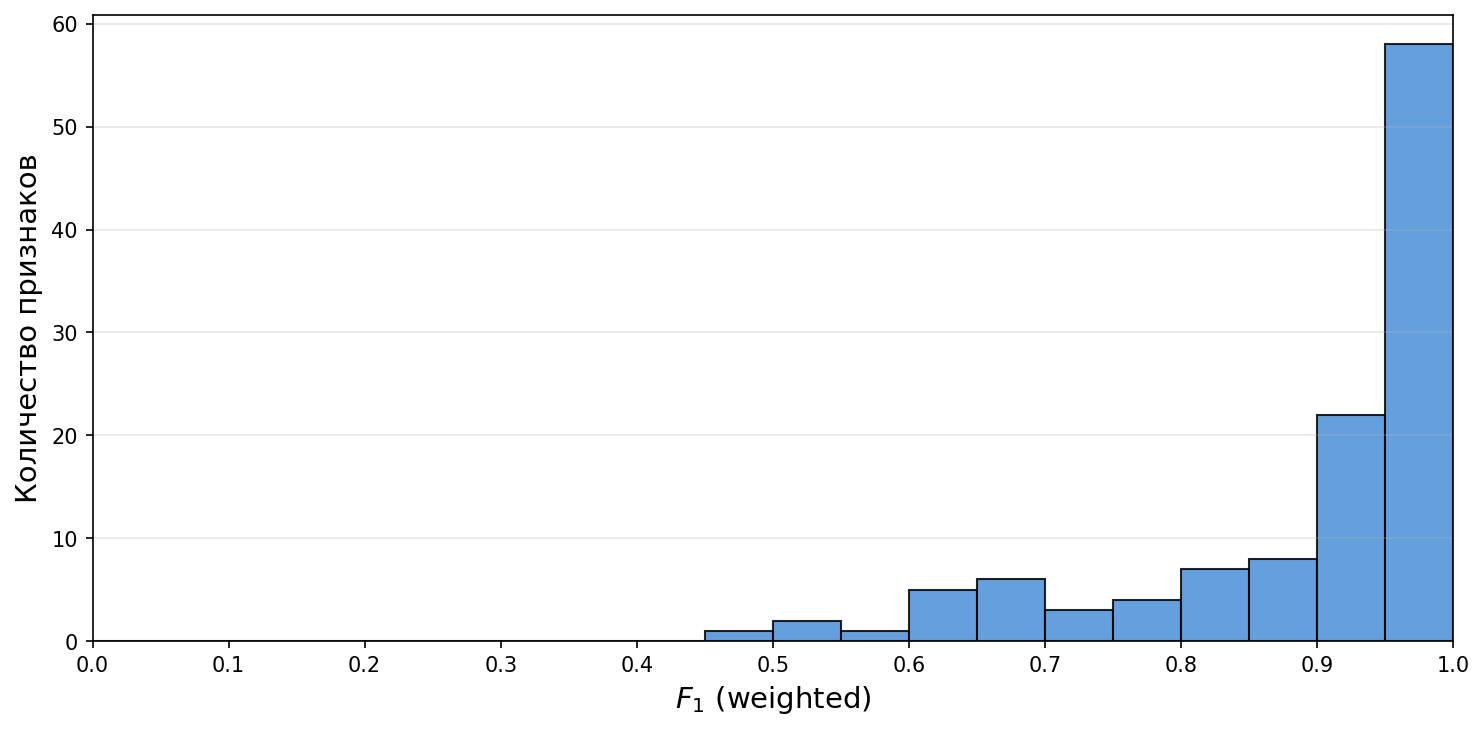
\includegraphics[width=0.85\linewidth]{inc/f1-distribution.png}
    \caption{Распределение F1\textsubscript{weighted} по 117 признакам}
    \label{fig:f1-distribution}
\end{figure}

Подавляющее большинство признаков имеет значение F1\textsubscript{weighted} в диапазоне 0,85--0,99, что подтверждает однородно высокое качество модели по совокупности задач.

Среди 117 признаков особо выделяются 10 признаков с экстремально малым числом положительных примеров (менее 10 в обучающей выборке). Для них объём данных принципиально не позволяет обучить классификатор, надёжно распознающий минорный класс: модель в большинстве случаев предсказывает мажоритарный класс, что обеспечивает высокое значение F1\textsubscript{weighted} (близкое к 1) и низкое значение F1\textsubscript{macro} (около 0,5). Эти признаки оказывают значительное влияние на среднее значение F1\textsubscript{macro} по всей выборке, но практически не влияют на F1\textsubscript{micro} и F1\textsubscript{weighted}.

В целом распределение метрик показывает, что модель успешно справляется с задачей классификации признаков рисунка для типичных рисунков. Снижение F1\textsubscript{macro} обусловлено редкими признаками, для которых при имеющемся объёме обучающих данных надёжная классификация минорного класса принципиально невозможна.

\subsection{Демонстрация работы программного комплекса}

Для демонстрации работы веб-сервиса загрузим рисунок из тестовой выборки через пользовательский интерфейс и проследим результат на каждом этапе конвейера.

На рисунке~\ref{fig:demo-header} представлена верхняя часть страницы результата: заголовок, метаинформация об анализе (число активных предсказаний, уникальный идентификатор), а также сравнение исходного отсканированного листа и результата предобработки --- кропированной и нормализованной фигуры.

\begin{figure}[h]
    \centering
    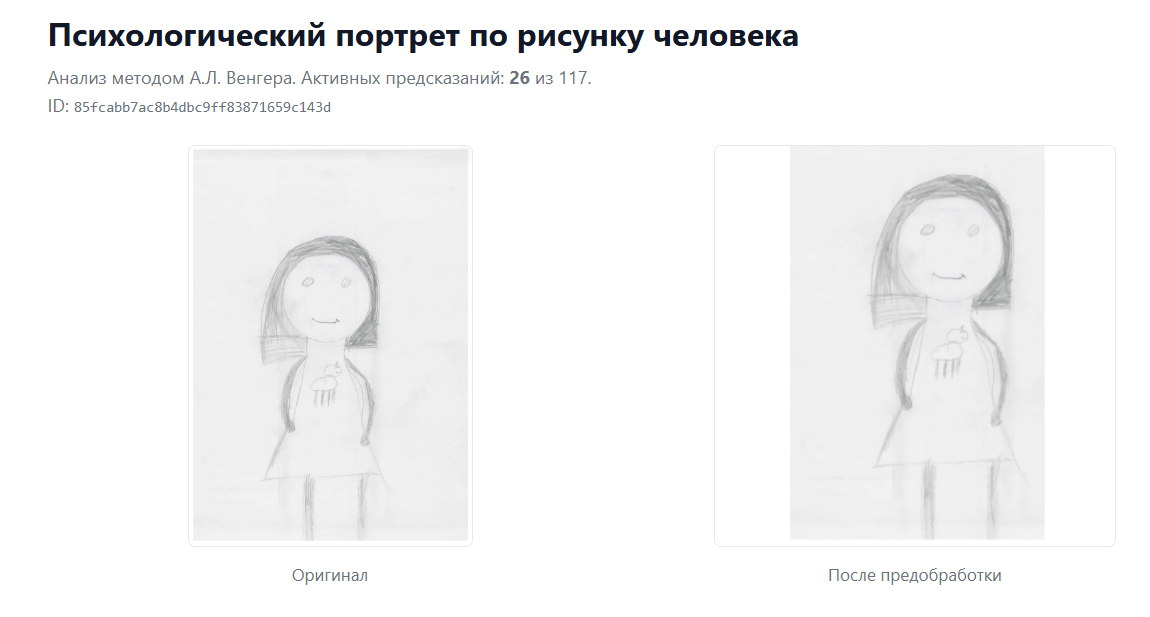
\includegraphics[width=0.8\linewidth]{inc/s1.png}
    \caption{Веб-интерфейс результата анализа: заголовок, метаданные и сравнение исходного изображения с результатом предобработки}
    \label{fig:demo-header}
\end{figure}

После прохождения изображения через нейросетевую модель 117 предсказаний транслируются через словарь интерпретаций в психологические черты. На рисунке~\ref{fig:demo-traits} показан раздел <<Ключевые особенности>> --- черты с поддержкой не менее двух признаков, ранжированные по степени выраженности. Для каждой черты указаны описание и список подтверждающих свидетельств.

\begin{figure}[h]
    \centering
    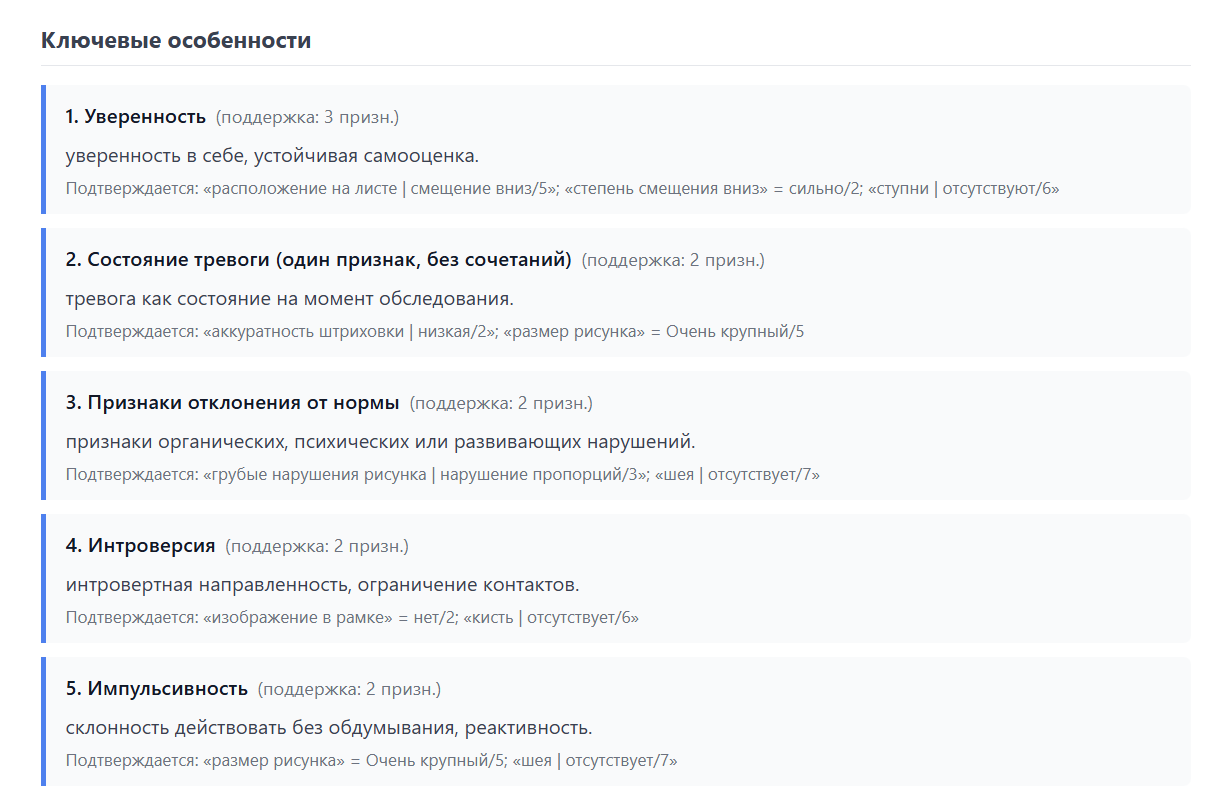
\includegraphics[width=0.8\linewidth]{inc/s2.png}
    \caption{Раздел <<Ключевые особенности>> сгенерированного психологического портрета}
    \label{fig:demo-traits}
\end{figure}

Помимо интерпретации, веб-интерфейс отображает технические детали работы модели. На рисунке~\ref{fig:demo-top10} приведена таблица десяти наиболее уверенных активных предсказаний с указанием имени признака, предсказанного значения и confidence (значение softmax).

\begin{figure}[h]
    \centering
    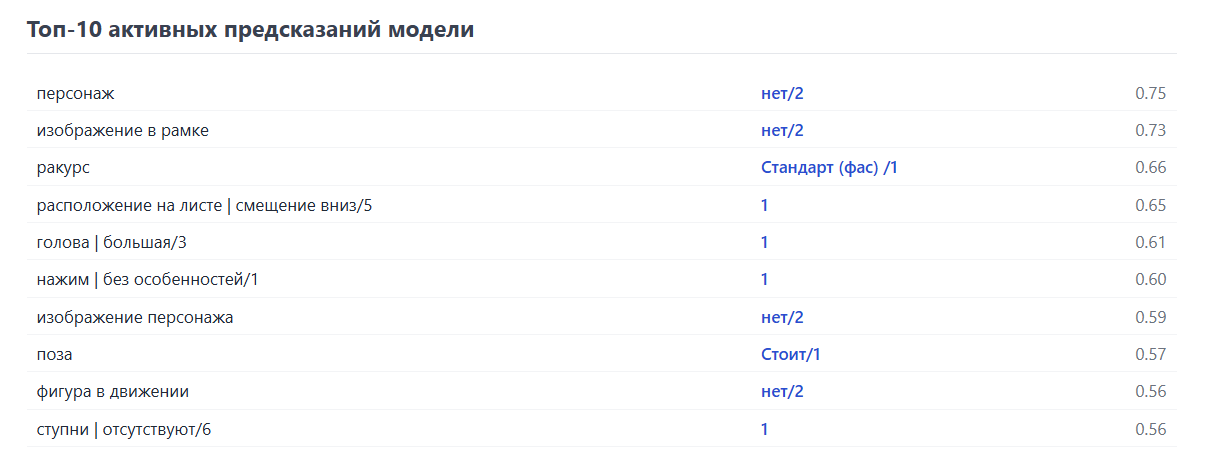
\includegraphics[width=0.8\linewidth]{inc/s3.png}
    \caption{10 активных предсказаний модели}
    \label{fig:demo-top10}
\end{figure}

\FloatBarrier
\subsection{Анализ временных характеристик}

Измерены характеристики времени работы программного комплекса в инференс-режиме на NVIDIA Tesla T4. Обработка одного рисунка от подачи на вход сырого изображения до возврата итогового текстового портрета занимает в среднем около 0,4~секунды. Это время разбивается на следующие компоненты:

\begin{itemize}
    \item чтение и декодирование изображения из файла --- около 0,05~с;
    \item локализация фигуры (адаптивная бинаризация, морфология, выделение связных компонент, фильтрация и объединение) --- около 0,15~с;
    \item кроп, паддинг, ресайз --- менее 0,01~с;
    \item инференс --- около 0,18~с (один прямой проход на одном изображении);
    \item декодирование 117 предсказаний и применение словаря интерпретаций --- менее 0,01~с;
    \item ранжирование черт и формирование итогового текста --- менее 0,01~с.
\end{itemize}

При пакетной обработке (batch inference) среднее время на один рисунок снижается за счёт лучшего использования параллелизма GPU: при обработке пакета из 32 рисунков время на одно изображение составляет около 0,05~секунд.

Время обучения модели от начала до завершения --- порядка 30--50~минут на одном NVIDIA Tesla T4 (50 эпох с ранней остановкой). Размер сохранённого чекпоинта --- около 22~МБ. Эти характеристики делают разработанный комплекс полностью применимым в практических условиях: при наличии современного GPU психолог может обработать пакет из сотен рисунков за несколько минут.

\subsection{Тестирование веб-сервиса}

Для верификации корректной работы микросервисной системы в целом проведено функциональное и нагрузочное тестирование развёрнутого веб-сервиса. Тестирование выполнялось на локальной машине (CPU: Intel Core i5, 16~ГБ ОЗУ) в режиме Docker-контейнеров без GPU.

Функциональное тестирование. Проверена корректность работы полного конвейера end-to-end: загрузка изображения через веб-форму, прохождение всех этапов обработки, формирование психологического портрета и сохранение результата в базу данных. Протестированы следующие сценарии:

\begin{itemize}
    \item загрузка типичного отсканированного рисунка формата A4 (2480$\times$3508, $\sim$1~МБ) --- успешная обработка, портрет сгенерирован;
    \item загрузка фотографии рисунка с мобильного устройства (4032$\times$3024, $\sim$3~МБ) --- успешная обработка;
    \item загрузка изображения без фигуры (чистый лист) --- система возвращает портрет без выраженных особенностей;
    \item загрузка файла некорректного формата --- корректная обработка ошибки с информативным сообщением;
    \item повторный просмотр сохранённого анализа по идентификатору --- портрет загружается из БД без повторного инференса.
\end{itemize}

Измерение времени отклика. Время обработки одного запроса (от отправки файла до получения HTML-портрета) при последовательной обработке составляет:

\begin{table}
    \caption{Время обработки одного рисунка через веб-сервис (CPU-режим)}
    \fontsize{12pt}{18pt}\selectfont
    \begin{tabular}{|l|c|}\hline
        \textbf{Этап} & \textbf{Время, с} \\ \hline
        Предобработка (OpenCV-локализация)    & 0,3--0,5 \\ \hline
        Вычисление bbox-признаков             & $<$\,0,01 \\ \hline
        Нейросетевой инференс (CPU)           & 1,5--2,5 \\ \hline
        Интерпретация и формирование портрета & $<$\,0,05 \\ \hline
        Сохранение в MinIO и PostgreSQL       & 0,1--0,2 \\ \hline
        Итого end-to-end                      & 2,0--3,2 \\ \hline
    \end{tabular}
    \label{tab:response-time}
\end{table}

Основное время занимает инференс на CPU. При развёртывании с GPU (NVIDIA Tesla T4) время инференса сокращается до $\sim$0,2~с, а общее время отклика --- до $\sim$0,7~с.

Нагрузочное тестирование. При параллельной отправке 10 запросов в секунду система обрабатывает все запросы без ошибок с линейным ростом латентности (запросы ставятся в очередь к единственному экземпляру сервиса инференса). При необходимости обслуживания большего числа одновременных пользователей достаточно горизонтально масштабировать сервис инференса (запуск нескольких реплик через Docker Compose).

Тестирование устойчивости. Проверена реакция системы на аварийные ситуации: при принудительной остановке контейнера \texttt{inference} API-шлюз возвращает корректное сообщение об ошибке; после перезапуска контейнера система восстанавливает работоспособность без ручного вмешательства благодаря директиве \texttt{restart: unless-stopped}. История ранее выполненных анализов остаётся доступной, поскольку хранится в PostgreSQL.

\subsection{Сфера применения и ограничения}

Разработанный программный комплекс может применяться психологами, педагогами и исследователями детской психологии в следующих сценариях.

Первый --- предварительный скрининг в детских садах и школах. Психолог может пропустить пакет рисунков через систему за минуты вместо часов и получить ранжированный список рисунков, требующих более детального индивидуального анализа.

Второй --- исследовательские задачи, в которых требуется обработка больших коллекций рисуночных тестов. Например, выявление средних тенденций в группе по полу или возрасту, корреляций психологических характеристик с социальными факторами, динамики изменения психологических черт со временем.

Третий --- учебные курсы по практической психологической диагностике. Система может применяться для демонстрации связи признаков рисунка с психологическими интерпретациями.

Среди ограничений разработки следует отметить следующие:

\begin{enumerate}
    \item система предназначена исключительно для теста <<Рисунок человека>> и не может быть напрямую применена к другим рисуночным тестам (<<Дом-Дерево-Человек>>, <<Несуществующее животное>>, <<Моя семья>> и др.) без переобучения. Возможна адаптация архитектуры для других тестов при наличии аналогичной обучающей выборки;
    \item выводы системы носят гипотетический характер и не могут заменить непосредственное общение специалиста с ребёнком, сбор анамнеза и наблюдение за ребёнком в естественных условиях. Психологический портрет, сгенерированный системой, является лишь предварительной гипотезой и должен подтверждаться независимыми источниками;
    \item точность предсказаний для редко встречающихся признаков объективно ограничена объёмом обучающих данных и требует осторожной интерпретации. Если итоговый портрет содержит черту, поддерживаемую только одним признаком, имеет смысл отнестись к ней с осторожностью; черты, поддерживаемые тремя и более признаками, существенно более надёжны;
    \item система обучена на рисунках детей дошкольного и младшего школьного возраста (приблизительно 5--12 лет). Для рисунков существенно других возрастных групп (подростков и взрослых) качество предсказаний может оказаться ниже, поскольку их рисуночные продукты имеют другие стилистические особенности;
    \item применение системы требует наличия отсканированного или сфотографированного рисунка достаточного качества. Сильно повреждённые, размытые или с фрагментированной фигурой изображения могут давать неустойчивые предсказания.
\end{enumerate}

Указанные ограничения не препятствуют практическому применению системы при учёте описанных условий и интерпретации её выводов как вспомогательных, а не окончательных.
